\section{计算成本与方法比较}
\label{sec:opt-sto-cost}

本章的方法可以归为四类计算安排：减少每步读取（随机梯度、非均匀抽样、小批量），复用历史信息（SVRG、SAGA与各种自适应统计），限制每步更新的范围（坐标下降与交替最小化），以及改变方向本身（裁剪、符号、矩阵整形、替代梯度）。要比较它们，必须先让原目标、返回对象和精度要求一致，再用同一个预算口径计数。本节给出这个口径，并说明在什么情况下哪一项成本才是真正的瓶颈。

\paragraph{计数单位与登记项目}
四种单位常被混用：一次梯度读取（求一个$\nabla f_i$）、一次参数更新、一次全数据遍历（$n$次读取）和一次完整分块循环（每块各更新一次）。随机梯度一次更新读$1$项，梯度下降读$n$项，SVRG的外循环读$n+2m$项，块坐标下降的一次完整循环在最小二乘上约等于一次梯度的计算量。除读取之外，还要登记方法特有的成本：快照的完整梯度、梯度表与统计量的存储、矩阵求根与分解、子问题的求解以及抽样分布的维护。表~\ref{tab:opt-sto-costs}汇总本章各方法的这些项目。

\begin{table*}[!htbp]
  \centering
  \caption{本章方法的每步成本与本章给出的保证。$n$为项数，$d$为参数维数，矩阵参数为$m\times d$，$b$为批量，$m_{\mathrm{in}}$为SVRG内循环长度。“读取”按单项梯度计。保证一栏只列本章正文实际给出或引用的结论及其主要条件。}
  \label{tab:opt-sto-costs}
  \footnotesize
  \begin{tabularx}{\linewidth}{@{}l>{\raggedright\arraybackslash}p{24mm}>{\raggedright\arraybackslash}p{20mm}>{\raggedright\arraybackslash}p{26mm}>{\raggedright\arraybackslash}X@{}}
    \toprule
    方法 & 每次更新读取 & 额外状态 & 额外计算 & 本章的保证（主要条件）\\
    \midrule
    梯度下降 & $n$ & — & — & 对照基准（第~\ref{chap:opt-smooth}章）\\
    随机梯度 & $1$ & — & — & 噪声邻域、$1/t$与$1/\sqrt T$速率（无偏、矩条件）\\
    非均匀抽样 & $1$ & 分布$O(n)$ & 抽样$O(1)$至$O(\log n)$ & 同上，常数由$p$决定（反比权重）\\
    小批量 & $b$ & — & — & 噪声项除以$b$（批内条件独立）\\
    SVRG & $2$，每外循环另加$n$ & $O(d)$ & — & 外循环线性收敛（每项凸光滑、$f$强凸）\\
    SAGA & $1$，初始化$n$ & $O(nd)$梯度表 & — & 线性收敛（同上，引用）\\
    AdaGrad、RMSProp & $1$ & $O(d)$ & $O(d)$ & 依具体分析而定（引用）\\
    Adam、AMSGrad & $1$ & $O(2d)$ & $O(d)$ & 依具体分析而定（引用）\\
    Adafactor & $1$ & $O(m+d)$ & $O(md)$重建 & 存储压缩；收敛另需论证\\
    Shampoo & $1$ & $O(m^2+d^2)$ & 求根$O(m^3+d^3)$/刷新 & 凸在线分析（引用）\\
    Lion & $1$ & $O(d)$ & $O(d)$ & 无一般保证；位移长$\eta\sqrt q$\\
    Muon & $1$ & $O(md)$动量 & $5$次迭代$O(md\min(m,d))$ & 无一般保证\\
    随机块坐标 & 一块的偏梯度 & — & 维护残差 & 强凸时线性收敛（块光滑）\\
    交替最小化 & 子问题所需 & — & 子问题求解 & 目标单调；块最优（附加条件）\\
    \bottomrule
  \end{tabularx}
\end{table*}

\paragraph{先固定误差对象}
不同方法的结论针对不同的误差对象：期望目标差、到最小点的期望距离、梯度平方残差的平均，或者带证书的目标差上界。返回对象也不同：最后一点、加权平均点、随机返回点。比较时应先选定一个误差对象和一个返回规则，对每种方法计算达到同一精度的总成本，而不是比较每步成本，也不是比较外层迭代次数。SVRG的一个外循环和随机梯度的一步完全不可比；Shampoo的一次参数更新若带一次矩阵求根，也不能与Adam的一次更新等量齐观。

\paragraph{抽样误差何时成为主要限制}
由定理~\ref{thm:opt-sto-constant-step}，常数步长随机梯度的误差由两部分组成：随迭代几何衰减的初始误差，以及大小约为$2\eta\sigma_\star^2/(b\mu)$的噪声平台。若目标精度远高于平台，噪声就是主要限制，此时增大批量与缩小步长等价，都要付出更多读取；若目标精度低于平台，噪声并不是问题，限制来自曲率，增大批量只是浪费。图~\ref{fig:opt-sto-batch-cost}把这一点画成曲线：在$n=10000$的最小二乘上，对每个批量$b$取最优的常数步长，计算期望目标差首次达到$10^{-3}$所需的读取量。$b\leq64$时读取量几乎不变，约$4.1\times10^4$，批量增大$b$倍，所需步数也减少约$b$倍；$b$超过数百后，最优步长已增大到$1/L$附近并逼近稳定上限$2/L$，步数不能再按比例减少，读取量随之上升，$b=4096$时约为$1.4\times10^5$。梯度下降需要$4.3\times10^5$次读取。这条曲线中“平坦段”到“上升段”的转折，就是噪声主导与曲率主导的分界。

\begin{figure}[!htbp]
  \centering
  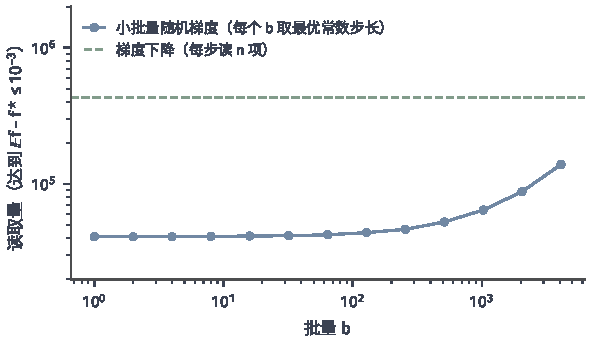
\includegraphics[width=100mm]{figures/03-optimization-evolution-and-signals/01-optimization/matplotlib/c6-batch-cost/figure.pdf}
  \caption{达到同一精度所需的读取量随批量的变化。岭回归最小二乘，$n=10000$，$d=5$，$\lambda=10^{-2}$，$L\approx1.00$，$\mu\approx0.050$，初值$\bm0$。蓝线：小批量随机梯度（有放回抽样），每个$b$在$80$个候选常数步长中取最优者，读取量指期望目标差首次不超过$10^{-3}$时已读取的样本数；期望由一阶与二阶矩的精确递推算出，没有蒙特卡罗误差。绿色虚线：步长$1/L$的梯度下降，$43$步、每步读$n$项。双对数坐标。}
  \label{fig:opt-sto-batch-cost}
\end{figure}

\paragraph{内层精度、批量与记忆的代价}
同样的推理适用于子问题。交替最小化或块邻近步骤中，如果子问题误差远小于外层每轮的改善，继续解准子问题没有意义；如果子问题误差与外层改善同量级，它就像偏差一样形成误差下限（第~\ref{sec:opt-sto-reading-error}节），此时解准内层才有回报。方差缩减与增大批量是两种降噪的代价形式：前者用$O(d)$的快照加周期性的全数据遍历，或用$O(nd)$的梯度表，换取线性收敛；后者用每步$b$倍的读取换取$1/b$的噪声。数据可以反复访问、$n$不太大时前者通常更省；数据流式到来或存储受限时，只能用后者。

\paragraph{比较时必须保持一致的约定}
最后，几个容易被忽略的约定会直接改变比较结果。目标是否除以$n$决定了光滑常数与梯度的量级，从而决定步长的数值，所以报告步长时要说明目标的归一化方式。停止准则要相同：一种方法按梯度范数停止，另一种按目标估计停止，二者不可比。返回对象要相同：用平均点评价一种方法、用最后一点评价另一种，会把返回规则的差异误当作方法的差异。在这些约定一致之后，读取、计算与存储的总量才是有意义的比较依据。
